近年、コンピューターの処理速度の向上やデータのデジタル化による扱えるデータの巨
大化などの要因に後押しされ、機械学習の分野の発展は大変著しい。この機械学習の技術を
用いて上記の極端降雨現象の予測に対する新しいアプローチの模索が行われている。

降雨のような時空間データを学習させるための機械学習モデルとしてShi \textit{et al}.[2015]
によってConvLSTM(Convolutional Long-Short Term Memory)が発表された。ConvLSTMは空間的な
特徴を学習させるための機械学習モデルであるCNN(Convolutional Neural Network, Hubel and Wiesel.[1962])と、時間的な
変化を学習させるためのモデルであるLSTM(Long-Short Term Memory, Hochreiter and Schmidhuber.[1997])を組み合わせた機械学習モデル
である。具体的な計算式は以下の通りである。

\begin{gather}
  i_{t} = \sigma\left(W_{xi} * X_{t} + W_{hi} * H_{t−1} + W_{ci} \odot \mathcal{C}_{t−1} + b_{i}\right)\label{eq:convlstm1} \\ 
  f_{t} = \sigma\left(W_{xf} * X_{t} + W_{hf} * H_{t−1} + W_{cf} \odot \mathcal{C}_{t−1} + b_{f}\right)\label{eq:convlstm2} \\
  \mathcal{C}_{t} = f_{t} \odot \mathcal{C}_{t−1} + i_{t} \odot \tanh\left(W_{xc} * X_{t} + W_{hc} * \mathcal{H}_{t−1} + b_{c}\right)\label{eq:convlstm3} \\
  o_{t} = \sigma\left(W_{xo} * X_{t} + W_{ho} * \mathcal{H}_{t−1} + W_{co} \odot \mathcal{C}_{t} + b_{o}\right)\label{eq:convlstm4} \\
  \mathcal{H}_{t} = o_{t} \odot \tanh\left(C_{t}\right)\label{eq:convlstm5} 
\end{gather}

さらにConvLSTMの内部構造の概念図以下に示す。

\begin{figure}[H]
\begin{center}
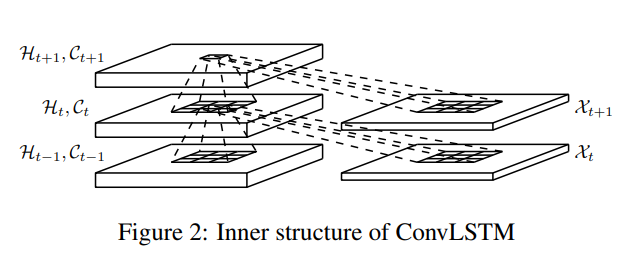
\includegraphics[width=0.9\linewidth]{fig/intro/inner-structure-of-convlstm.png}
\captionsetup{width=0.9\linewidth}
\caption{ConvLSTMの内部構造の概念図。Shi \textit{et al}.[2015] Figure2より引用。ConvLSTMの内部構造の概念図。}
\label{fig:convlstm-inner-structure}
\end{center}
\end{figure}

図\ref{fig:convlstm-inner-structure}の$\mathcal{X}_{t}$・$\mathcal{C}_{t}$・$\mathcal{H}_{t}$はそれぞれ入力・セル状態・
隠れ層の出力を表しており、上記の計算式における$X_{t}$・$C_{t}$・$H_{t}$と対応している。
入力は各時刻における入力される空間データを示す。セル状態は過去の状態に関する情報を蓄積
する働きをする。このセル状態が時系列データの効率的な学習を可能としている。計算式(\ref{eq:convlstm1})
の$i_{t}$は入力ゲートと呼ばれ、入力$X_{t}$と1つ前の時刻の出力$H_{t-1}$に対して畳み込み演算($*$)
が施された結果と1つ前の時刻のセル状態$C_{t-1}$が重み付けされた結果の和をシグモイド関数
を用いて正規化している。さらに計算式(\ref{eq:convlstm2})の$f_{t}$は忘却ゲートと呼ばれ入力ゲートと同様の計算
が行われれるが、重み$W$が異なっている。計算式(\ref{eq:convlstm3})の右辺第1項は先ほど求めた忘却ゲートを用いて
過去のセル状態を調整している。右辺第2項は入力ゲートを用いて入力$X_{t}$と1つ前の時刻の出力
$H_{t-1}$の和を調整している。計算式(3)は最終的にこれらを用いてセル状態を更新していること
がわかる。$\odot$はアダマール積を示す。計算式(\ref{eq:convlstm4})の$o_{t}$は出力ゲートと呼ばれており、
計算式(\ref{eq:convlstm5})で最終的な出力$H_{t}$を求る際に更新されたセル状態$C_{t}$を調整する働きをしている。

Shi \textit{et al}.[2015]ではモデルの提案に加え、降雨のレーダーエコー画像を入力として
ConvLSTMモデルを学習させ一定時間後の降雨の分布と強度を予測する実験も行われた。その結果
を図\ref{fig:shi-et-al-table2}に示す。

\begin{figure}[H]
\begin{center}
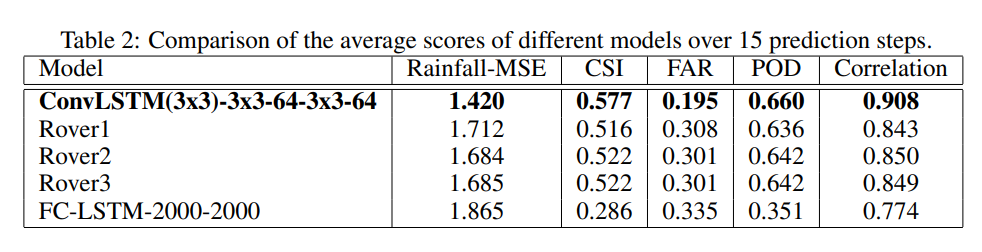
\includegraphics[width=0.9\linewidth]{fig/intro/shi-et-al-convlstm-mse-table.png}
\captionsetup{width=0.9\linewidth}
\caption{Shi \textit{et al}.[2015] Table2より引用。ConvLSTM、ROVER、FC-LSTMにおける降雨の予測精度の比較結果。}
\label{fig:shi-et-al-table2}
\end{center}
\end{figure}

図\ref{fig:shi-et-al-table2}の通り、従来手法の1つであるROVER(Real-time Optical flow by Variational methods for Echoes of Radar)
を比較した結果、ConvLSTMモデルは従来手法よりも高い精度で降雨の分布と強度を予測できた。ROVER1・2・3は
モデルの初期化条件を3つのパターンに分けた場合のそれぞれのROVERモデルである。FC-LSTM(fully connected 
LSTM)はLSTMのみを用いて予測するモデルである。Rainfall-MSEは予測値と実測値とのMean Squared Error(平均2乗誤差)
、CSI・FAR・PODはそれぞれCritial Success Index・False Alarm Ratio・Probability of Detectionを示す。0.5mm/h
以上の降雨が観測OR予測された場合に1、それ以外の場合を0としてそれぞれCSI・FAR・PODを計算した。

この論文が発表されて以来、ConvLSTMを用いた降雨予測の研究が盛んに行われた。Su \textit{et al}.[2020]
の研究ではConvLSTMに降雨のレーダーエコー画像データだけでなく東西・南北風成分を同時に学習させることで
予測のより困難な局所的な対流が原因の降雨の強度や分布の変化を予測できる可能性が示された。本論文の
学習プロセスの概要図を図\ref{fig:su-et-al-fig2}に示す。

\begin{figure}[H]
\begin{center}
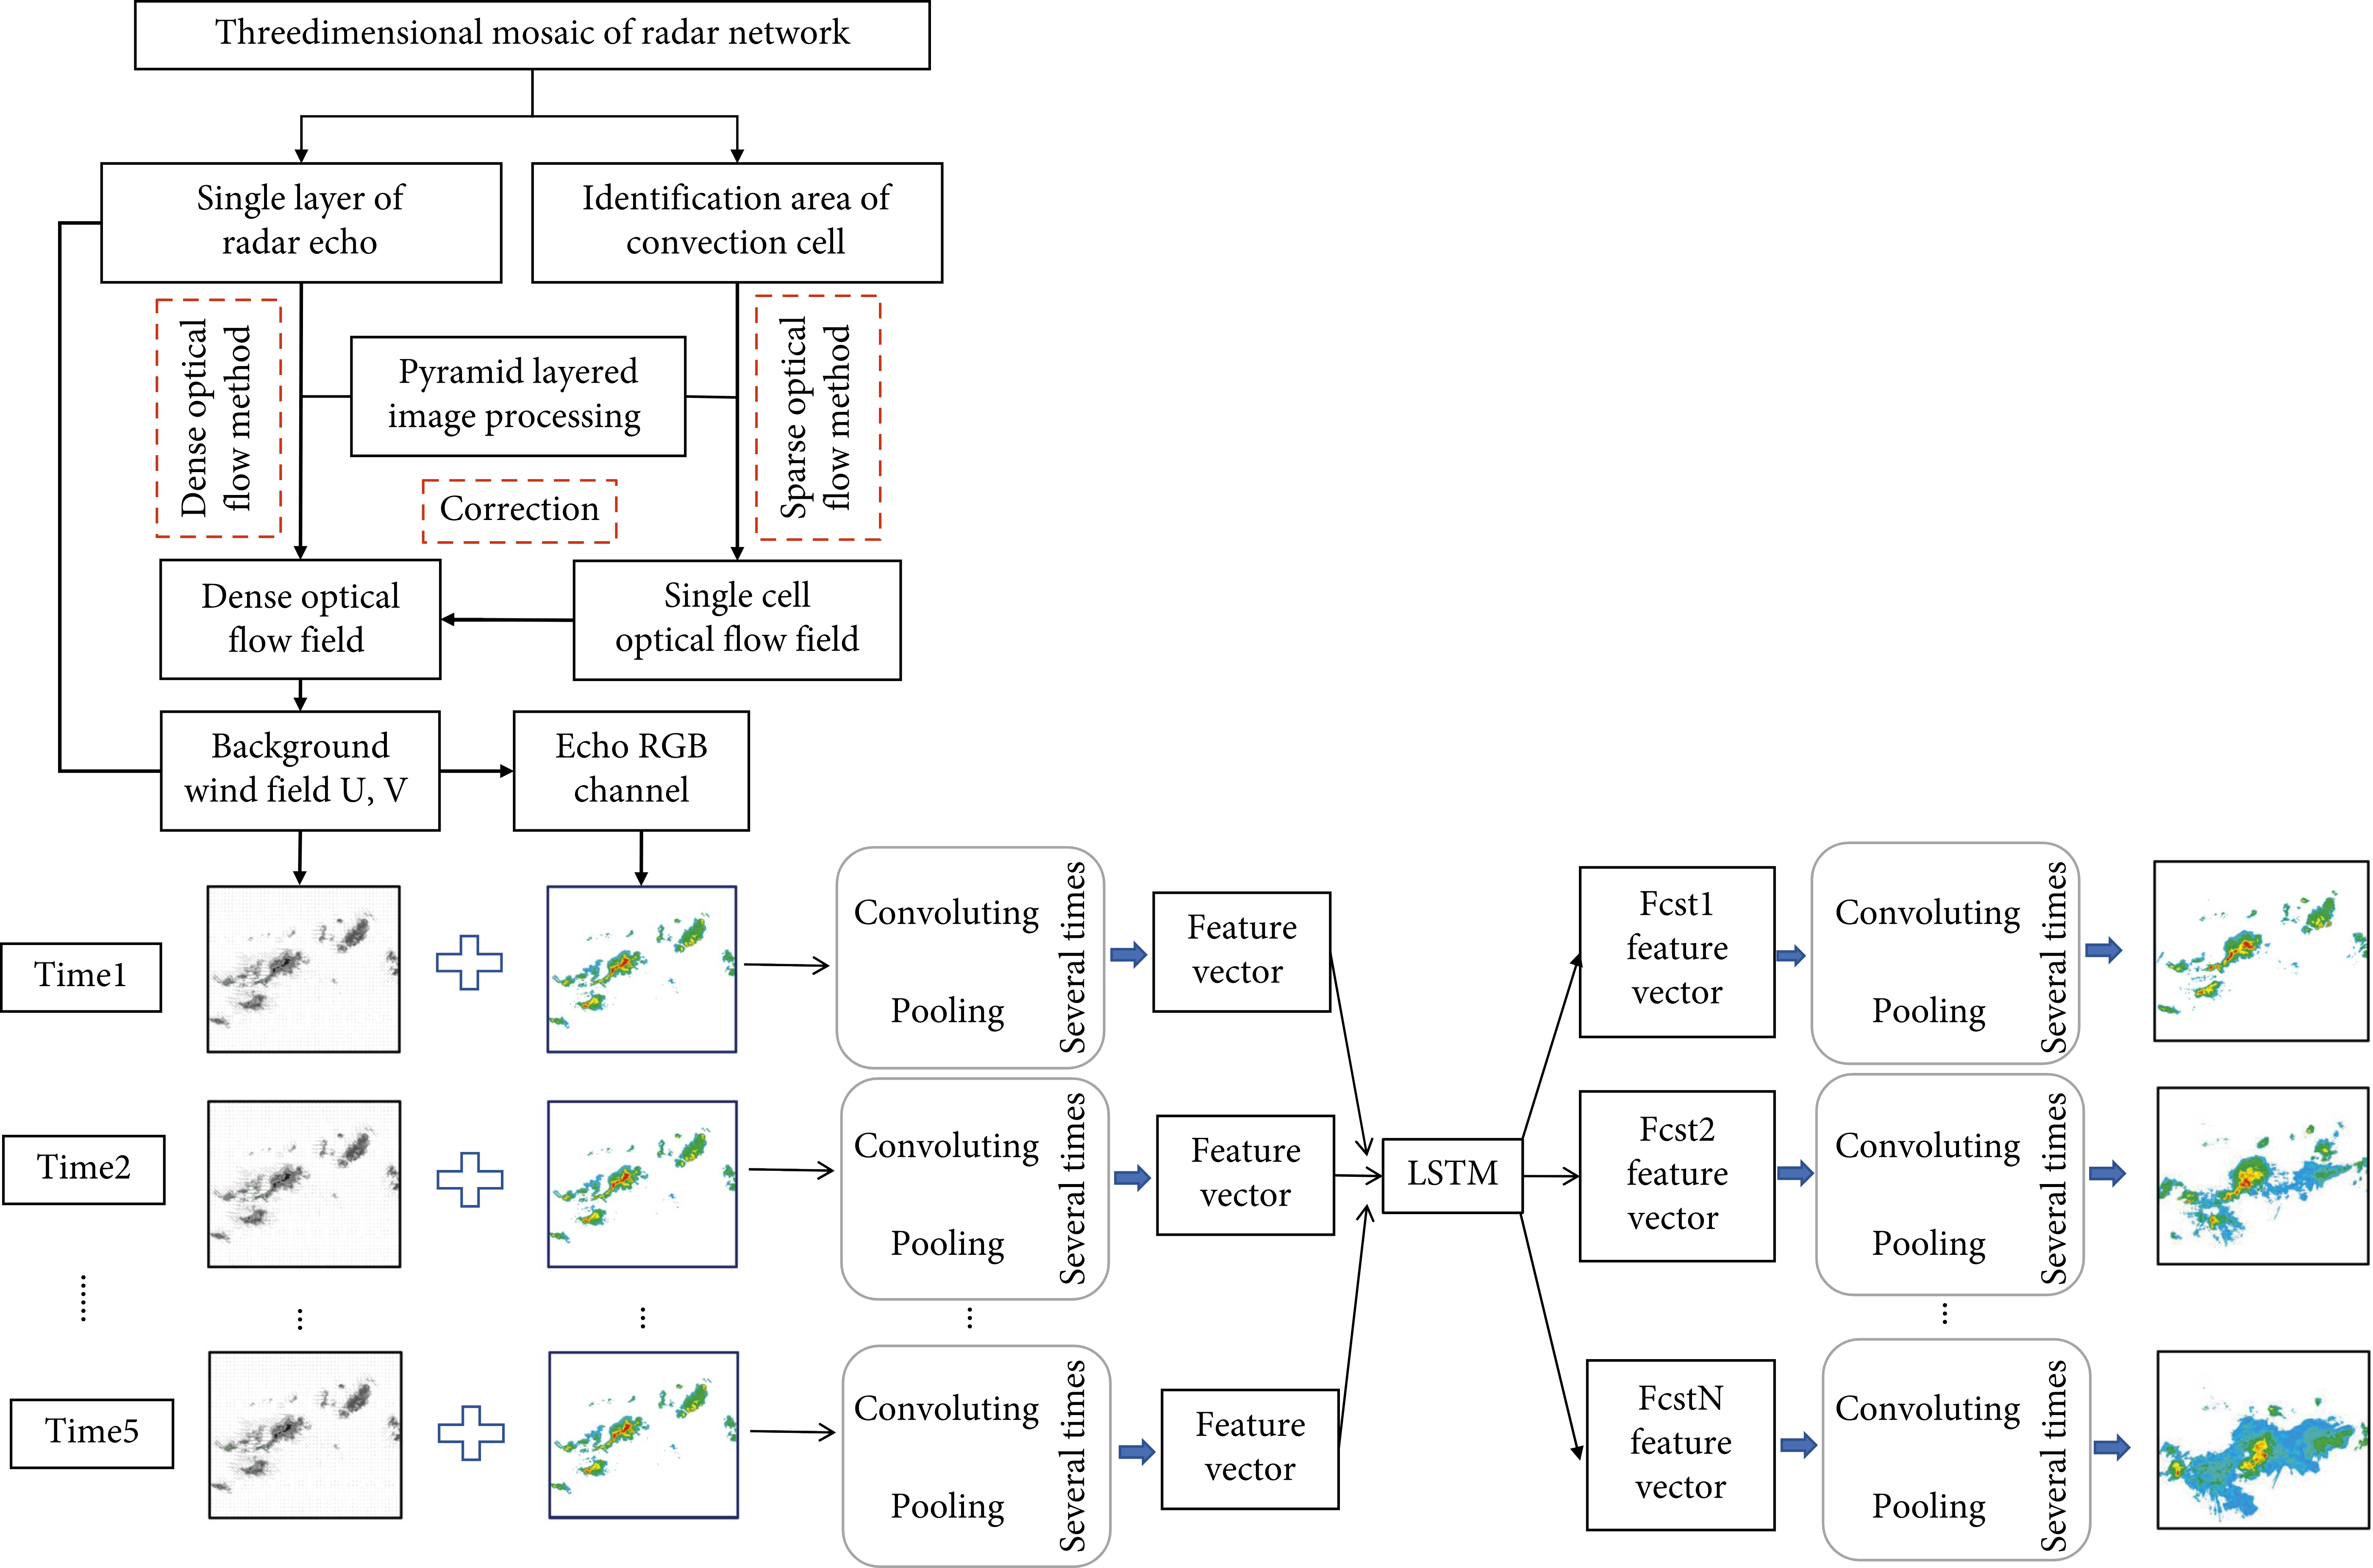
\includegraphics[width=0.9\linewidth]{fig/intro/su-et-al-flowchart.png}
\captionsetup{width=0.9\linewidth}
\caption{Su \textit{et al}.[2020] Figure2より引用。降雨と東西・南北風データをConvLSTMに学習させるプロセスの概念図。}
\label{fig:su-et-al-fig2}
\end{center}
\end{figure}

以下の図\ref{fig:su-et-al-fig6}はSu \textit{et al}.[2020]の予測結果の1つである。

\begin{figure}[H]
	\begin{tabular}{cc}
		\begin{minipage}[t]{1.0\hsize}
		\begin{center}
		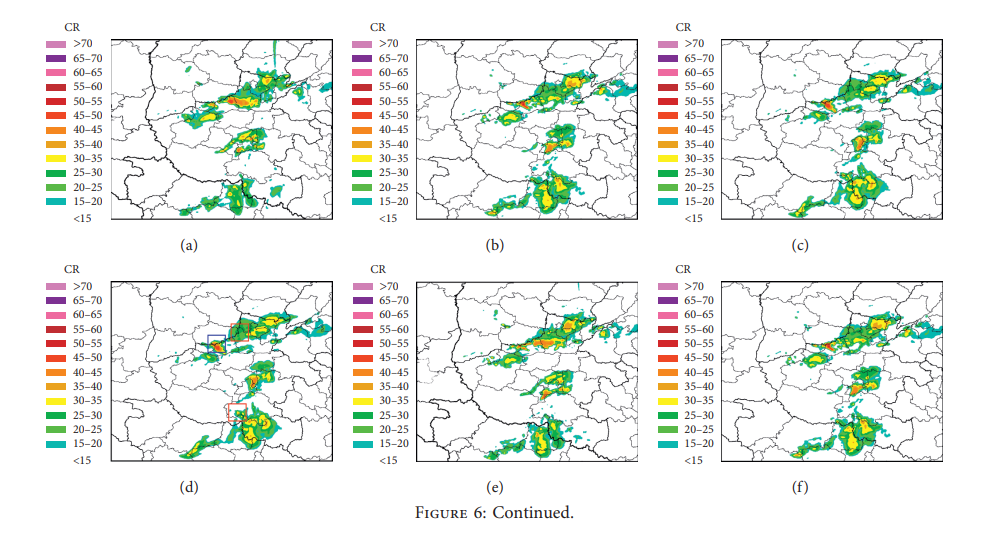
\includegraphics[width=0.9\linewidth,clip]{fig/intro/su-et-al-fig6-1.png}
		\label{a}
		\end{center}
		\end{minipage}\\
		
		\begin{minipage}[t]{1.0\hsize}	
		\begin{center}
		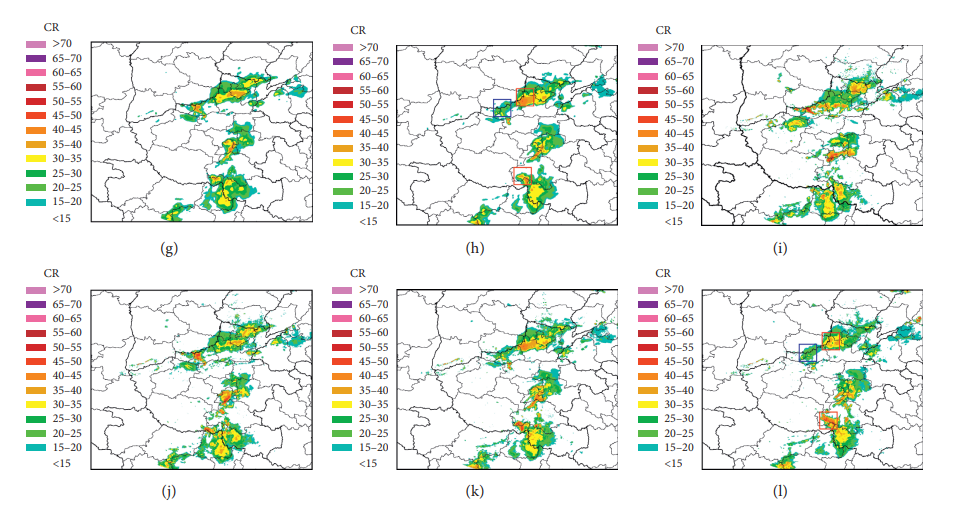
\includegraphics[width=0.9\linewidth,clip]{fig/intro/su-et-al-fig6-2.png}
		\label{b}
		\end{center}
		\end{minipage}
	\end{tabular}
	\captionsetup{width=0.9\linewidth}
	\caption{Su \textit{et al}.[2020] Figure6より引用。従来手法であるオプティカルフローでの30分・60分・90分・120分後の予測がそれぞれ(a)・(b)・(c)・(d)。ConvLSTMでの30分・60分・90分・120分後の予測がそれぞれ(e)・(f)・(g)・(h)。降雨の30分・60分・90分・120分後の実測画像がそれぞれ(i)・(j)・(k)・(l)。}
	\label{fig:su-et-al-fig6}
\end{figure}

図\ref{fig:su-et-al-fig6}の従来手法の予測結果(d)とConvLSTM予測結果(h)、降雨の実測画像(l)の赤枠と
青枠はそれぞれConvLSTMが予測でき、従来手法は予測できなかった部分とその逆の場合の部分を示している。
このケースのみならず多くの場合において雨だけでなく風と共に学習させたConvLSTMの方が降雨の強い部分を
より多く予測できた結果となった。降雨とそれに関連する気象パラメータを一緒に学習させることで、従来手
法では予測が難しかった降雨を予測できる可能性を示した。

Shi \textit{et al}.[2015]の発表以降、ConvLSTMの発表をベースにして様々な時空間データを学習させるた
めの機械学習モデルが提案された。PredRNN (Wang \textit{et al}.[2017b])は水平方向だけでなく鉛直方向
成分を持つ時空間データを扱うために新しいセル状態を導入した。これによって空間のダイナミクスに関する
情報をより効率的に学習可能となった。さらにWang \textit{et al}.[2018b])にてPredRNNを改良した
PredRNN++が提案された。Wang \textit{et al.}[2019]では定常・非定常の情報を処理するためにより多くのメ
モリセルを導入したことで、より高次元のダイナミクスを学習することに成功したMemory in Memory (MIM)モ
デルが提案された。同論文内では多大な計算コストが必要とはなるもののMIMモデルが時空間予測における当時の最高
レベルの予測性能を達成したことが示された。そしてSelf-Attention ConvLSTM (Lin \textit{et al}.[2020])
が発表され、ConvLSTMやPredRNN++、MIMなどといった他の時空間予測モデルよりも高いベンチマークスコアを
記録したことが示された(図\ref{fig:lin-et-al-movingmnist})。このモデルではSelf-Attention機構を導入
したことで畳み込み処理では扱えなかったデータ全域に渡る特徴を捉えることができるようになった。さら
に過去のSelf-Attention機構の状態を新しく追加したメモリーモジュールで保管・更新することで時系列に適
したモデルとして拡張した。

\begin{figure}[H]
\begin{center}
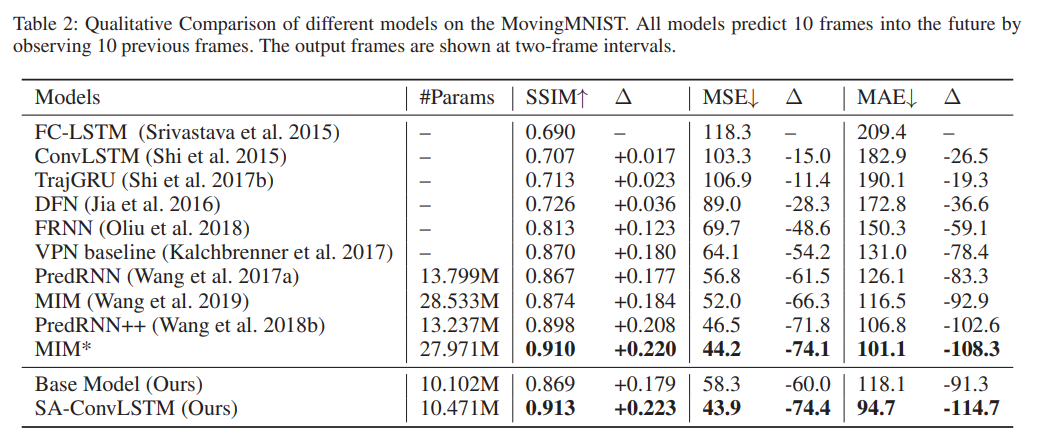
\includegraphics[width=0.9\linewidth]{fig/intro/lin-et-al-movingmnist.png}
\captionsetup{width=0.9\linewidth}
\caption{Lin \textit{et al}.[2020] Table2より引用。Self-Attention ConvLSTMと他モデルとのMovingMNIST(手書き数字の時系列移動データセット)に対する予測性能の比較。}
\label{fig:lin-et-al-movingmnist}
\end{center}
\end{figure}

このモデルで新しく導入されたSelf-Attention機構は、その計算方法から空間内のある1点と他のすべての点との関連度合い
を計算する。またその関連度合いは人間でも解釈が可能であり、今までブラックボックスとなっていたモデルの内部状態
を知ることができる。この関連度合いはアテンションマップと呼ばれ、Lin \textit{et al}.[2020]の論文内でもその結果が
示されていた(図\ref{fig:lin-et-al-attention-map})。

\begin{figure}[H]
\begin{center}
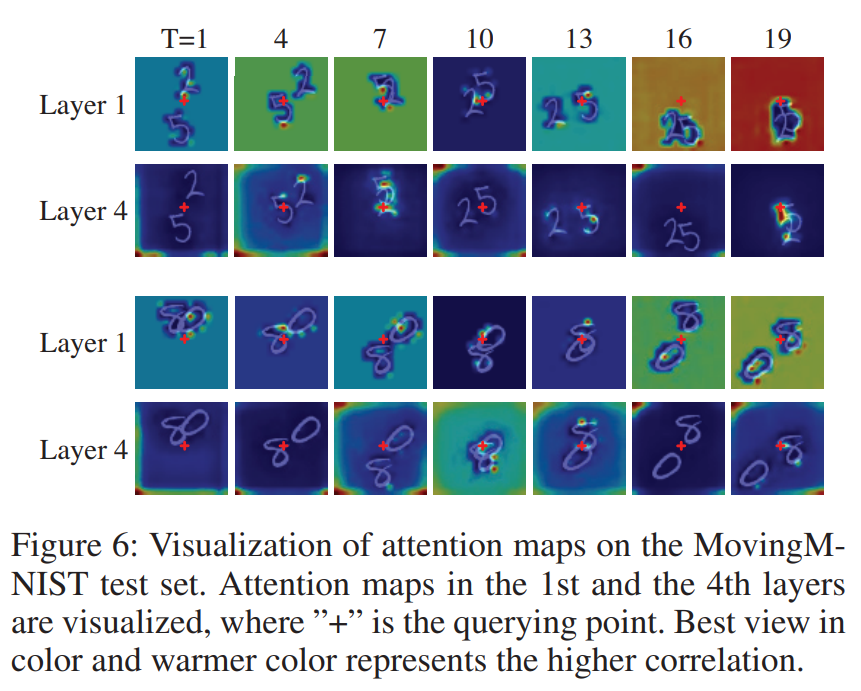
\includegraphics[width=0.9\linewidth]{fig/intro/lin-et-al-attention-map.png}
\captionsetup{width=0.9\linewidth}
\caption{Lin \textit{et al}.[2020] Figure6より引用。あるケースにおけるSelf-Attention ConvLSTMのアテンションマップを可視化した図。Layer1・4はそれぞれ多層に重ねたSelf-Attention ConvLSTMモデルの1層目・4層目を示す。空間内の赤い十字マークの点とそれ以外の点との関連度合いを色で示している。Tは時間ステップを示す。赤に近い色ほど関連度合いが高く、青いほど関連度合いが低い。}
\label{fig:lin-et-al-attention-map}
\end{center}
\end{figure}

図\ref{fig:lin-et-al-attention-map}から、"T=13"や"T=19"に注目すると層が深くなればなるほど赤十字マーク
(クエリポイント)と同じ部分である手書き文字の部分にアテンションが高まっていることがわかる。またクエリ
ポイントが背景部分にある場合("T=1"や"T=16"など)は層が深くなるほど背景に注目が移っていくことがわかる。
このアテンションマップの可視化からこの手書き文字のデータセットにおいて、Self-Attention機構は手書き文字
の部分と背景部分を区別して注目することを可能にし、学習性能を向上させたことがわかった。このようにAttention
機構を取り入れたことによって性能改善だけでなく機械学習モデルの説明可能性も向上したことは注目すべき点である。